\chapter[SCP-044 二战分子裂变炮]{
    SCP-044 World War II Era Molecular-Fission Cannon\\
    SCP-044 二战分子裂变炮
}

\label{chap:SCP-044}

\begin{figure}[H]
    \centering
    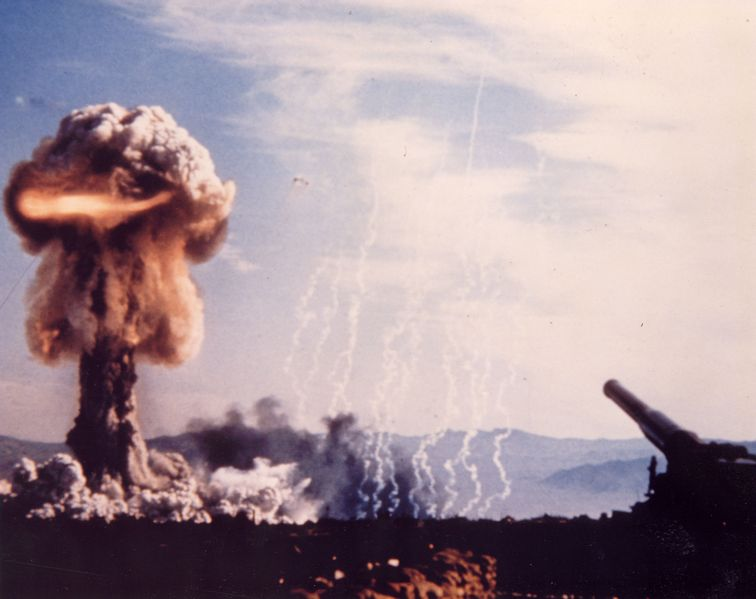
\includegraphics[width=0.5\linewidth]{images/SCP-044.jpg}
    \caption*{在一次被命名为“Upshot Knolte Ford Grable”的实验中拍摄到的SCP-044的图像}
\end{figure}

\bb{项目编号:}SCP-044

\bb{项目分类:}Safe

\bb{特殊收容措施:}在SCP-044的炮口处,有一股由氢离子,初生态氧原子,以及其他自由基粒子组成的射流持续不停地喷出。因此在SCP-044的坞站内应保持良好通风以防有害气体和湿气聚积。炮口护幕应一直保持遮盖以防禽鸟或小动物进入SCP-044宽大的炮管中觅食。

\bb{附录██\slash ██\slash 200█:}鉴于SCP-044已经有█年未曾卷入由基金会引起的重大事件,SCP-044被重归类为Safe。

\ii{我何必要给“重大事件”下定义?要是遵守收容章程和标准安全协议,044估计不会比任何其他的大█炮更危险。呃不,“Bear”事件不算。}\\
–O5-██

\bb{描述:}SCP-044是一门短管式榴弹炮,由克虏伯兵工厂的工程师在第二次世界大战晚期秘密制造,由阿道夫希特勒统治时期的德国军工装备部部长阿尔伯特·施佩尔监督。SCP-044其特殊之处不仅在于其尺寸(达251000公斤,或251吨),而且还因为它的非常规火力,其火炮使用一种非常规的发射方式:并非是使用后膛来容纳弹壳装药与弹头,而是在它炮管后部配备有一个巨大的空压舱。任何物体,或任何一堆物体都能被当作炮弹\slash 装药装填到空压仓内。由于其硕大无比,SCP-044只能在铁轨上运输和部署并且需要两台动力机车头来拖动。

研究人员认为SCP-044可以降低任何装填入空压仓中的物质的分子或原子间作用力。然而SCP-044这种影响分子键的技术尚未探明,因为SCP-044的外壳和工作方式都是由众多复杂的零件和机制组成的。事实上SCP-044的某些机件似乎根本就是没用的,只会旋转或者发出噪音,甚至并未启动SCP-044的时候也是如此(尚不知其能量来源为何)。已经在探索SCP-044炮体内部时失去了两批设备和人员。

SCP-044发射时,其炮管内部的物质化为一种炽热的高速率弹头射出,其总尺寸与塞入炮管的物质总量成正比。在击中一个固体目标或者是地面时,弹头将会爆炸,经测量爆炸当量相当于成比例份量的原始火药,其物质能量转化效率不低于███\%。随着弹头在炮体中放置得更久,其份量也会有所增加。其最大已知当量,是在把‘管理人员的’8900公斤(19500磅)的私人柴油敞蓬小型载货卡车整个塞入SCP-044的炮管并且开炮时达到的,图中为该次试验。
